\documentclass{beamer}

\usepackage{hyperref}
\usepackage{bm}
\usepackage{tikz}

\newcommand{\q}[1]{``#1''} 
\newcommand{\mycite}[1]{{\scriptsize \color{blue} \autocites{#1}}}
\newcommand{\bluebold}[1]{{\color{blue} \textbf{#1}}}
\newcommand{\redbold}[1]{{\color{red} \textbf{#1}}}

\usetikzlibrary{matrix,decorations.pathreplacing,calc}
\usetheme{Madrid}

\DeclareMathOperator*{\argmin}{\arg\!\min}
\DeclareMathOperator*{\argmax}{\arg\!\max}

%\let\olditem\item
%\renewcommand{\item}{\setlength{\itemsep}{\fill}\olditem}

\newenvironment{fitemize}[2]%
{%
\vspace{#1} %
\begin{itemize} \setlength{\itemsep}{#2}%
}%
{\end{itemize}}

\newenvironment{fenumerate}[2]%
{%
\vspace{#1} %
\begin{enumerate} \setlength{\itemsep}{#2}%
}%
{\end{enumerate}}


\usecolortheme{whale}

% Don't show things we don't want to see
\beamertemplatenavigationsymbolsempty
%\hypersetup{pdfpagemode=UseNone} % don't show bookmarks on initial view

% Slide number in lower right
\definecolor{gray}{RGB}{155,155,155}
\setbeamertemplate{footline}{%
    
\includegraphics[width=2cm,trim={0 6cm 0 7cm},clip]{IST_A_CMYK_POS.pdf}%
    \hfill%
    \raisebox{5pt}{
    \makebox{%
        \color{gray}%
        \scriptsize%
        \insertframenumber\,/\,\inserttotalframenumber\kern1em%
    }%
    }%
\hspace*{5pt}}

% Space between paragraphs on notes page
\addtobeamertemplate{note page}{\setlength{\parskip}{12pt}}

% Color and shape of bullets
%\setbeamercolor{item}{fg=gray} 
%\setbeamercolor{subitem}{fg=gray}
%\setbeamercolor{itemize/enumerate subbody}{fg=gray}
%\setbeamertemplate{itemize item}{{\textendash}}
%\setbeamertemplate{itemize subitem}{{\textendash}}
%\setbeamerfont{itemize/enumerate subbody}{size=\footnotesize}
%\setbeamerfont{itemize/enumerate subitem}{size=\footnotesize}

\usepackage{amssymb,amsmath}
\usepackage{ifxetex,ifluatex}
\usepackage{fixltx2e} % provides \textsubscript
\ifxetex
  \usepackage{fontspec,xltxtra,xunicode}
  \defaultfontfeatures{Mapping=tex-text,Scale=MatchLowercase}
\else
  \ifluatex
    \usepackage{fontspec}
    \defaultfontfeatures{Mapping=tex-text,Scale=MatchLowercase}
  \else
    \usepackage[utf8]{inputenc}
  \fi
\fi

% Comment these out if you don't want a slide with just the
% part/section/subsection/subsubsection title:
\AtBeginPart{
  \let\insertpartnumber\relax
  \let\partname\relax
  \frame{\partpage}
}
\AtBeginSection{
  \let\insertsectionnumber\relax
  \let\sectionname\relax
  \frame{\sectionpage}
}
\AtBeginSubsection{
  \let\insertsubsectionnumber\relax
  \let\subsectionname\relax
  \frame{\subsectionpage}
}

\setlength{\parindent}{0pt}
\setlength{\parskip}{6pt plus 2pt minus 1pt}
\setlength{\emergencystretch}{3em}  % prevent overfull lines
\setcounter{secnumdepth}{0}
\title{Variational Mixture of Normalizing Flows}
\author{Guilherme Grijó Pen Freitas Pires}

\usepackage[
    backend=biber,
    style=authoryear,
    sortlocale=en_EN,
    natbib=true,
    url=false,
    doi=true,
    eprint=false
]{biblatex}
\newrobustcmd*{\parentexttrack}[1]{%
  \begingroup
  \blx@blxinit
  \blx@setsfcodes
  \blx@bibopenparen#1\blx@bibcloseparen
  \endgroup}

\AtEveryCite{%
  \let\parentext=\parentexttrack%
  \let\bibopenparen=\bibopenbracket%
  \let\bibcloseparen=\bibclosebracket}

\makeatother
\addbibresource{presentation.bib}

\AtBeginSection[]
{
    \begin{frame}
        \frametitle{Table of Contents}
        \tableofcontents[currentsection]
    \end{frame}
}
\begin{document}
{
\begin{frame}[plain,noframenumbering]
  \titlepage
  \begin{center}
    \centering
    Thesis to obtain the Master of Science degree in \\
    \textbf{Electrical and Computer Engineering} \\
    \vspace{1cm}
    \footnotesize{Supervisor: Prof. Mário A. T. Figueiredo} \\
    
\includegraphics[width=3cm]{IST_A_CMYK_POS.pdf}
  \end{center}
\end{frame}
}

\hypertarget{introduction-and-motivation}{%
\section{Introduction and
Motivation}\label{introduction-and-motivation}}

\begin{frame}{Introduction and Motivation}
\protect\hypertarget{introduction-and-motivation-1}{}

\begin{fitemize}{0pt}{20pt}
\onslide<1->{\item Deep generative models: an active area of research}
    \begin{fitemize}{15pt}{15pt}
        \onslide<2->{\item \bluebold{Implicit distributions}: Generative adversarial networks
            \mycite{GAN}, Variational Autoencoder \mycite{vaepaper}
            \begin{fitemize}{10pt}{15pt}
                \item No explicit access to the density function \end{fitemize}}
        \onslide<3->{\item \bluebold{Explicit distributions}: Normalizing flows \mycite{shakir_nf}
            \begin{fitemize}{20pt}{15pt}
                \item Explicit access to the density function
                \item No approach to introduce discrete structure (multi-modality)
            \end{fitemize}}
    \end{fitemize}
\end{fitemize}

\end{frame}

\begin{frame}{Introduction and Motivation: Goal}
\protect\hypertarget{introduction-and-motivation-goal}{}

\begin{fitemize}{0pt}{25pt}
\onslide<1->{\item Goal of this work: \bluebold{mixture of flexible distributions}.}
\onslide<2->{\item Two questions:}
    \begin{fitemize}{15pt}{25pt}
        \onslide<3->{\item What should the \bluebold{mixture components} be?}
        \onslide<4->{\item How should their \bluebold{parameters} be \bluebold{estimated}?}
    \end{fitemize}
\end{fitemize}

\end{frame}

\begin{frame}{Outline}
\protect\hypertarget{outline}{}

\begin{fitemize}{0pt}{12pt}
\onslide<1->{\item Mixture Models}
\onslide<2->{\item Variational Inference}
    \onslide<3->{\begin{fitemize}{12pt}{12pt}
        \item The chosen framework for estimating the parameters of the proposed model\end{fitemize}}
\onslide<4->{\item Normalizing Flows}
    \onslide<5->{\begin{fitemize}{12pt}{12pt}
        \item The chosen family for the mixture model components \end{fitemize}}
\onslide<6->{\item Variational Mixture of Normalizing Flows}
\onslide<7->{\item Experiments and results}
\onslide<8->{\item Conclusions and future work}
\end{fitemize}

\end{frame}

\hypertarget{mixture-models}{%
\section{Mixture Models}\label{mixture-models}}

\begin{frame}{Mixture Models: Definition}
\protect\hypertarget{mixture-models-definition}{}

\begin{fitemize}{10pt}{10pt}
    \onslide<1->{\item Mixture model: used to model data that contains \bluebold{subgroups}.}
    \onslide<2->{\item \q{Subgroup-conditional} distributions (typically) in the same family}
\end{fitemize}
\onslide<3->{\centering 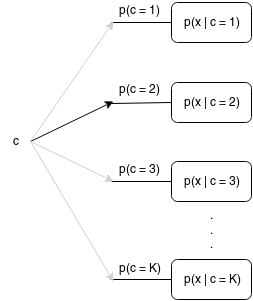
\includegraphics[width=0.3\textwidth]{figures/selector-mixture.png}}

\end{frame}

\begin{frame}{Mixture Models: Plate diagram}
\protect\hypertarget{mixture-models-plate-diagram}{}

\centering

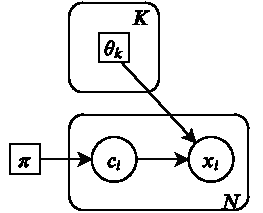
\includegraphics[width=0.5\textwidth]{figures/plate_diagram3.pdf}

\end{frame}

\begin{frame}{Mixture Models: Mixture of Gaussians}
\protect\hypertarget{mixture-models-mixture-of-gaussians}{}

\centering
\onslide<1->{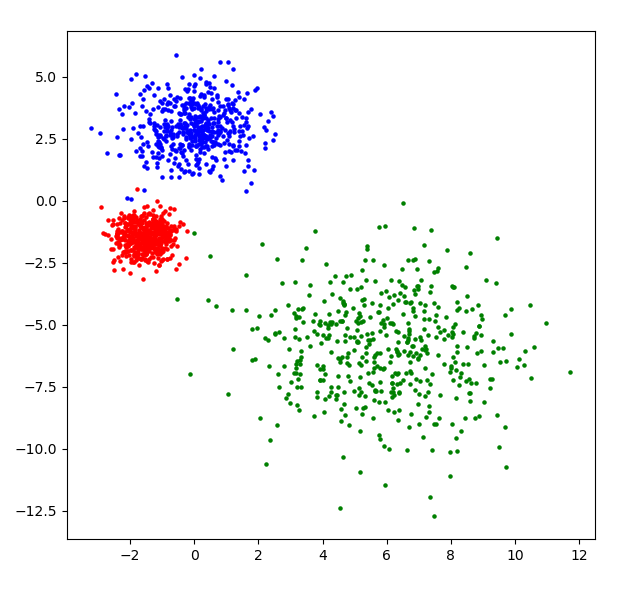
\includegraphics[width=0.475\textwidth]{figures/mog.png}}
\hfill
\onslide<2->{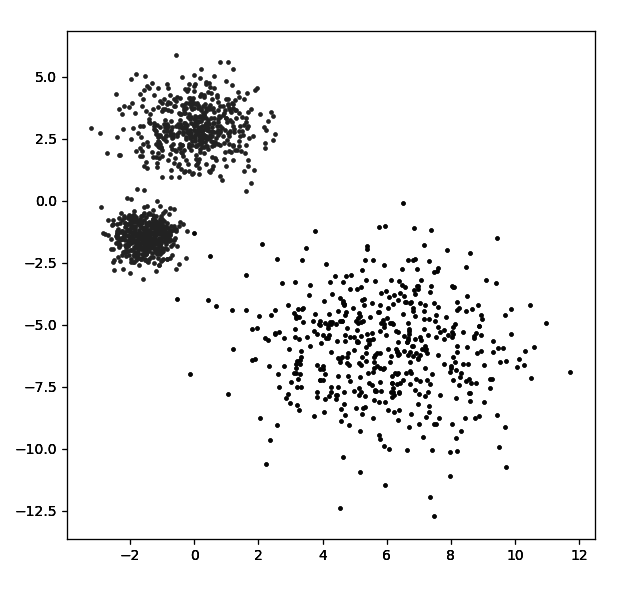
\includegraphics[width=0.475\textwidth]{figures/mog_observed.png}}

\end{frame}

\hypertarget{normalizing-flows}{%
\section{Normalizing Flows}\label{normalizing-flows}}

\begin{frame}{Normalizing Flows: Change of Variables}
\protect\hypertarget{normalizing-flows-change-of-variables}{}

\onslide<1->{Given
\begin{align*}
\begin{cases}
    \bm{z} \sim p(\bm{z}) \\
    \bm{x} = g(\bm{z}; \bm\theta)
\end{cases}
\end{align*}}
\onslide<2->{then:
\begin{align*}
    f_X(\bm{x}) &= f_Z(g^{-1}(\bm{x};\bm\theta))\Big|\det\Big(\frac{d}{d\bm{x}}g^{-1}(\bm{x};\bm\theta)\Big)\Big| \\
    &= f_Z(g^{-1}(\bm{x};\bm\theta))\Big|\det\Big(\frac{d}{d\bm{z}}g(\bm{z};\bm\theta) \bigg{|}_{\bm{z} = g^{-1}(\bm{x};\bm\theta)}\Big)\Big|^{-1}
\end{align*}}

\onslide<3->{This can be \bluebold{optimized w.r.t. $\bm\theta$}, to approximate an \bluebold{arbitrary distribution}}

\end{frame}

\begin{frame}{Normalizing Flows: Change of Variables}
\protect\hypertarget{normalizing-flows-change-of-variables-1}{}

\vspace{-20pt}
\onslide<1->{Requirements for feasibility}
\begin{fenumerate}{10pt}{30pt}
    \renewcommand{\theenumi}{\alph{enumi}}
    \onslide<2->{\item Base density - \bluebold{closed form} and \bluebold{easy to sample} from}
    \onslide<3->{\item \bluebold{Determinant} of the \bluebold{Jacobian} of $g$ - computationally cheap}
    \onslide<4->{\item \bluebold{Gradient} of $\det\Big(\frac{d}{d\bm{z}}g(\bm{z};\bm\theta)\Big)$ w.r.t $\bm\theta$ - computationally cheap}
\end{fenumerate}

\end{frame}

\begin{frame}{Normalizing Flows: Change of Variables}
\protect\hypertarget{normalizing-flows-change-of-variables-2}{}

\begin{fitemize}{0pt}{30pt}
\onslide<1->{\item Normalizing Flows: \bluebold{composition} of several \q{good} transformations}
\onslide<2->{\item I.e., \bluebold{$g = h_{L-1} \circ h_{L-2} \circ ... \circ h_1 \circ h_0$}}
\onslide<3->{\item Applying the formula to $g$, and taking the logarithm:
\begin{align*}
    \log f_X(\bm{x}) = \log f_Z(g^{-1}(\bm{x})) - \sum_{\ell=0}^{L-1} \log \Big|\det\Big(\frac{d}{d\bm{x_{\ell}}}h_{\ell}(\bm{x_\ell})\Big) \Big|. \label{eq:nflowsfinal}
\end{align*}}
\end{fitemize}

\end{frame}

\begin{frame}{Normalizing Flows: Affine Coupling Layer}
\protect\hypertarget{normalizing-flows-affine-coupling-layer}{}

\begin{fitemize}{0pt}{10pt}
\onslide<1->{\item An example: Affine Coupling Layer \mycite{real-nvp}}
\onslide<2->{\item Splitting $\bm{z}$ into $(\bm{z_1}, \bm{z_2})$,}
\onslide<3->{\begin{align*}
    \begin{cases}
    \bm{x_1} &= \bm{z_1} \odot \exp\big(s(\bm{z_2})\big) + t(\bm{z_2}) \\
    \bm{x_2} &= \bm{z_2}.
    \end{cases}
\end{align*}}
\onslide<4->{\item The respective Jacobian matrix:
\begin{align*}
    J_{f(z)} =
        \begin{tikzpicture}[decoration=brace, baseline=-\the\dimexpr\fontdimen22\textfont2\relax ]
            \matrix (m) [matrix of math nodes,left delimiter=[,right delimiter={]}, ampersand replacement=\&] {
                \mbox{\Large$\frac{\partial \bm{x_1}}{\partial \bm{z_1}}$} \& \mbox{\Large$\frac{\partial \bm{x_1}}{\partial \bm{z_2}}$} \\
                \mbox{\Large$\frac{\partial \bm{x_2}}{\partial \bm{z_1}}$} \& \mbox{\Large$\frac{\partial \bm{x_2}}{\partial \bm{z_2}}$} \\
            };
        \end{tikzpicture}
    =
        \begin{tikzpicture}[decoration=brace, baseline=-\the\dimexpr\fontdimen22\textfont2\relax ]
            \matrix (m) [matrix of math nodes,left delimiter=[,right delimiter={]}, ampersand replacement=\&] {
                \mbox{diag}\Big(\exp\big(s(\bm{z_2})\big)\Big) \& \mbox{\Large$\frac{\partial \bm{x_1}}{\partial \bm{z_2}}$} \\
                \mbox{\Large$\bm{0}$} \& \mbox{\Large$I$} \\
            };
        \end{tikzpicture}
\end{align*}
}
\end{fitemize}

\end{frame}

\hypertarget{variational-inference}{%
\section{Variational Inference}\label{variational-inference}}

\begin{frame}{Variational Inference: Preamble}
\protect\hypertarget{variational-inference-preamble}{}

\begin{fitemize}{0pt}{10pt}
\onslide<1->{\item Joint probability distribution $p(\bm{x}, \bm{c})$.}
\onslide<2->{\item $\bm{x}$ is observed and $\bm{c}$ is latent.}
\onslide<3->{\item Inference about $\bm{c}$, given $\bm{x}$, by \bluebold{Bayes' Law}:
\begin{align*}
    p(\bm{z}|\bm{x}) &= \frac{p(\bm{x}|\bm{c})p(\bm{c})}{p(\bm{x})} \\
                     &= \frac{p(\bm{x}|\bm{c})p(\bm{c})}{\int p(\bm{x}|\bm{c}')p(\bm{c'}) d\bm{c'}}
\end{align*}
}
\onslide<4->{\item Problem: The integral is normally \bluebold{intractable}}
\onslide<5->{\begin{fitemize}{10pt}{0pt} \item \bluebold{Variational inference}:
an \bluebold{approximate inference} framework to overcome this intractability. \end{fitemize}}
\end{fitemize}

\end{frame}

\begin{frame}{Variational Inference: Goal}
\protect\hypertarget{variational-inference-goal}{}

\centering

Given a family \(q(\bm{c} ; \bm\lambda)\), find the parameters
\(\bm{\lambda^{*}}\) such that: \begin{align*}
    \bm{\lambda^{*}} = \argmin_{\bm\lambda} KL(q(\bm{c}; \bm\lambda) || p(\bm{c} | \bm{x}))
\end{align*}

\end{frame}

\begin{frame}{Variational Inference: Goal}
\protect\hypertarget{variational-inference-goal-1}{}

\centering

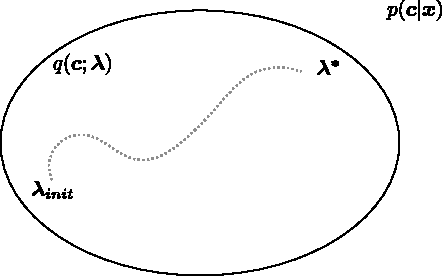
\includegraphics[width=0.7\textwidth]{figures/vi.pdf}

\end{frame}

\begin{frame}{Variational Inference: ELBO}
\protect\hypertarget{variational-inference-elbo}{}

\vspace{-20pt}

\begin{align*}
\onslide<1->{KL(q(\bm{c}) || p(\bm{z}|\bm{x})) &= \int q(\bm{c}) \log\frac{q(\bm{c})}{p(\bm{c}|\bm{x})} d\bm{c} \\}
\onslide<2->{&= \int q(\bm{c}) (\log q(\bm{c}) - \log p(\bm{c}|\bm{x})) d\bm{c} \\}
\onslide<3->{&= \int q(\bm{c}) (\log q(\bm{c}) - (\log p(\bm{x}, \bm{c}) - \log p(\bm{x}))) d\bm{c} \\}
\onslide<4->{&= \mathbb{E}_q [\log q(\bm{c})] - \mathbb{E}_q [\log p(\bm{x}, \bm{c})] + \log p(\bm{x})}
\end{align*} \onslide<5-> Which yields the lower bound (ELBO):
\begin{align*}
    \mbox{ELBO}(q) &= \mathbb{E}_q [\log p(\bm{x}, \bm{c})] - \mathbb{E}_q [\log q(\bm{c})] \\
            &= \mathbb{E}_q [\log p(\bm{x}|\bm{c})] + \mathbb{E}_q [\log p(\bm{c})] - \mathbb{E}_q [\log q(\bm{c})]
\end{align*}

\end{frame}

\hypertarget{variational-mixture-of-normalizing-flows}{%
\section{Variational Mixture of Normalizing
Flows}\label{variational-mixture-of-normalizing-flows}}

\begin{frame}{VMoNF: Introduction}
\protect\hypertarget{vmonf-introduction}{}

\onslide<1->{Is it possible to \bluebold{combine} the ideas from the previous sections,
to obtain a mixture of flexible models?}

\end{frame}

\begin{frame}{VMoNF: Definition}
\protect\hypertarget{vmonf-definition}{}

\begin{fitemize}{0pt}{20pt}
\onslide<1->{\item Recall the ELBO:
\begin{align*}
    ELBO(q) &= \mathbb{E}_q [\log p(\bm{x}|\bm{c})] + \mathbb{E}_q [\log p(\bm{c})] - \mathbb{E}_q [\log q(\bm{c})]
\end{align*}}
\onslide<2->{\item Parameterize $q(z|x)$ with a \bluebold{neural network}}
\onslide<3->{\item Optimize the ELBO, by \bluebold{jointly} learning the variational posterior and
the generative components.}
\end{fitemize}

\end{frame}

\begin{frame}{VMoNF: Overview}
\protect\hypertarget{vmonf-overview}{}

\centering

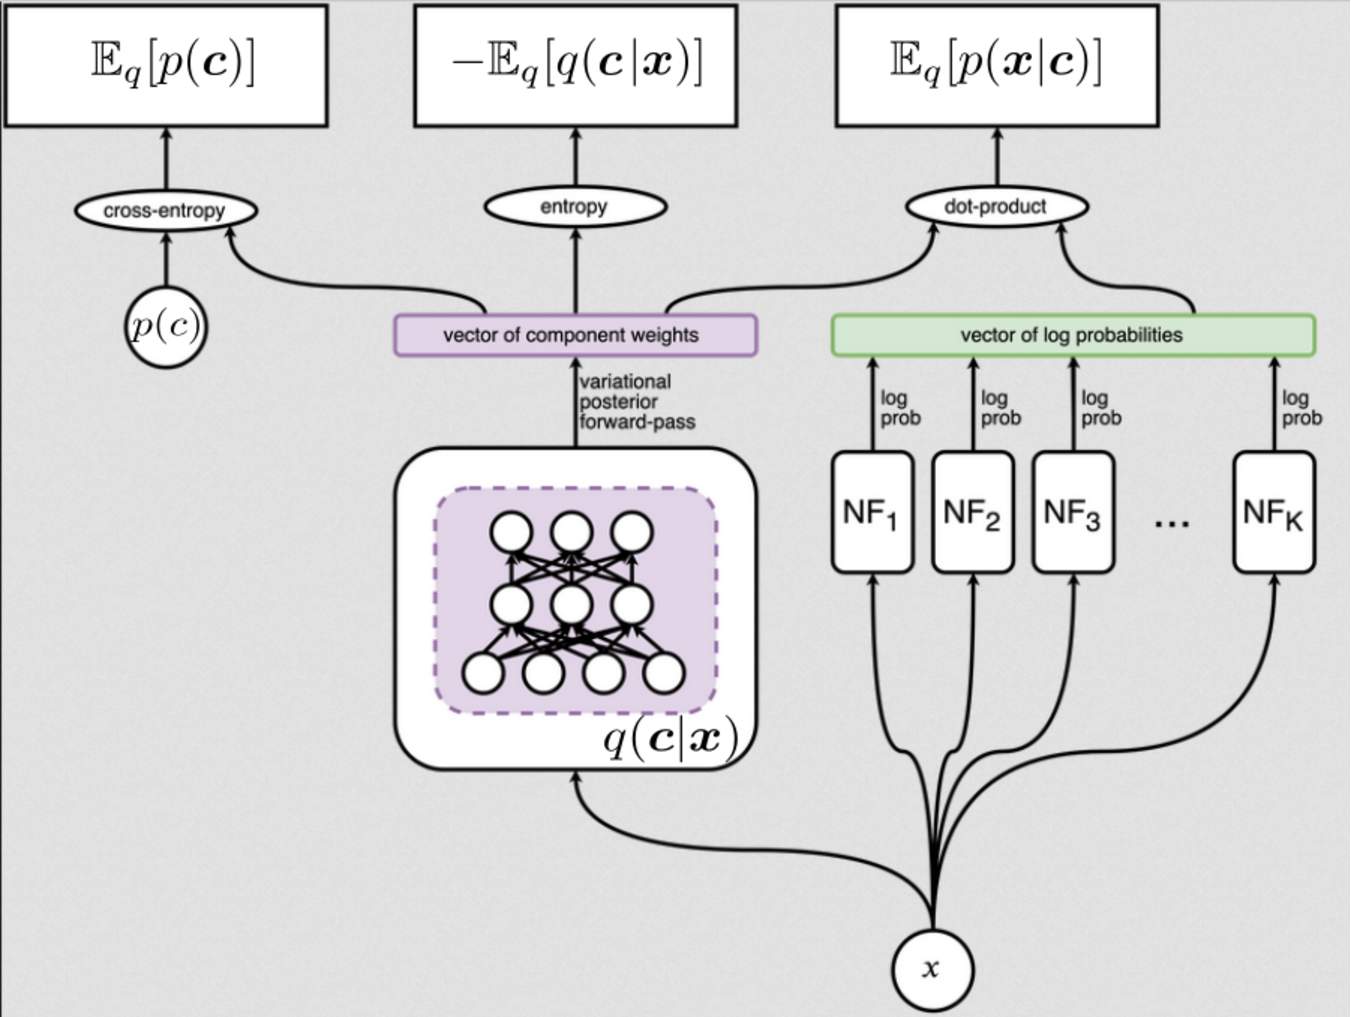
\includegraphics[width=0.7\textwidth]{figures/overview.pdf}

\end{frame}

\begin{frame}{VMoNF: Experiments - Pinwheel (5 wings)}
\protect\hypertarget{vmonf-experiments---pinwheel-5-wings}{}

\centering
\onslide<1->{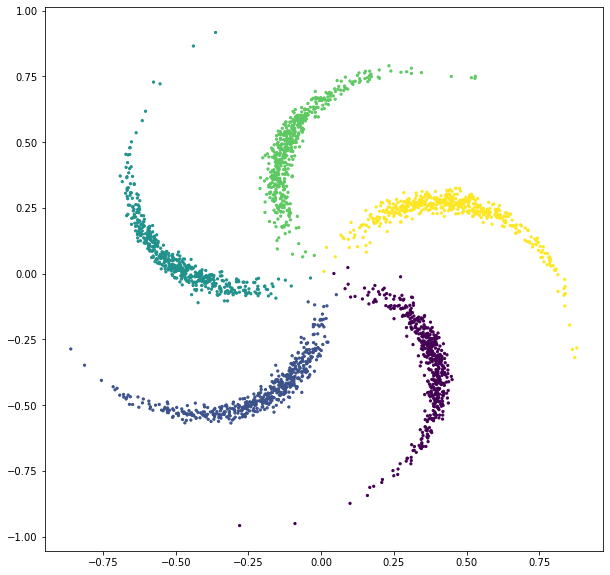
\includegraphics[width=0.475\textwidth]{figures/original_pinwheel.png}}
\hfill
\onslide<2->{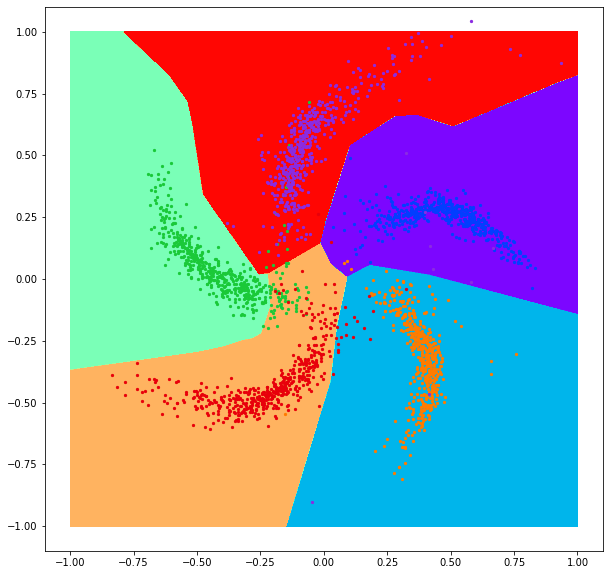
\includegraphics[width=0.475\textwidth]{figures/trained_pinwheel.png}}

\end{frame}

\begin{frame}{VMoNF: Experiments - Pinwheel (3 wings)}
\protect\hypertarget{vmonf-experiments---pinwheel-3-wings}{}

\centering

Trainining Animation

\end{frame}

\begin{frame}{VMoNF: Experiments - 2 Circles}
\protect\hypertarget{vmonf-experiments---2-circles}{}

\centering
\onslide<1->{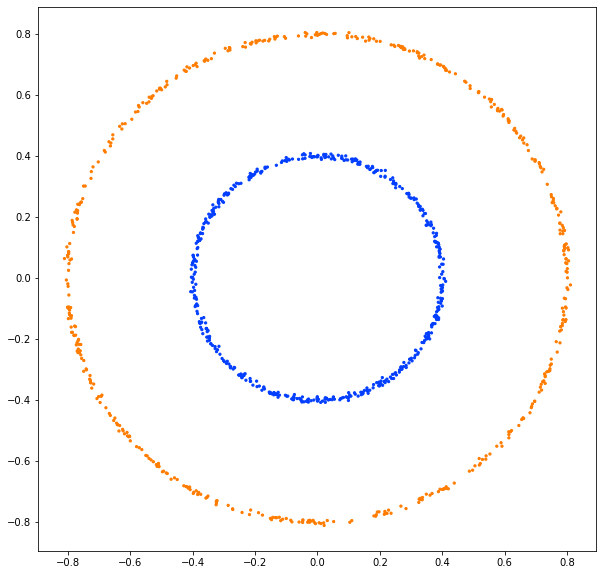
\includegraphics[width=0.475\textwidth]{figures/original_2_circles.png}}
\hfill
\onslide<2->{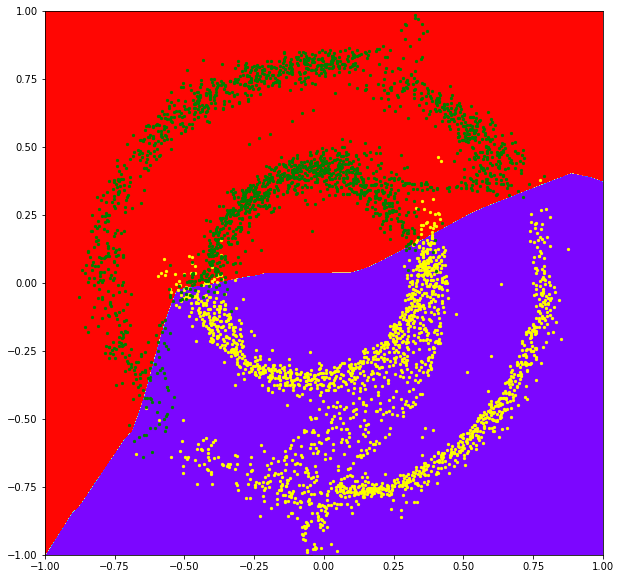
\includegraphics[width=0.475\textwidth]{figures/trained_2_circles_2.png}}

\end{frame}

\begin{frame}{VMoNF: Experiments - 2 Circles (semi supervised)}
\protect\hypertarget{vmonf-experiments---2-circles-semi-supervised}{}

\centering
\onslide<1->{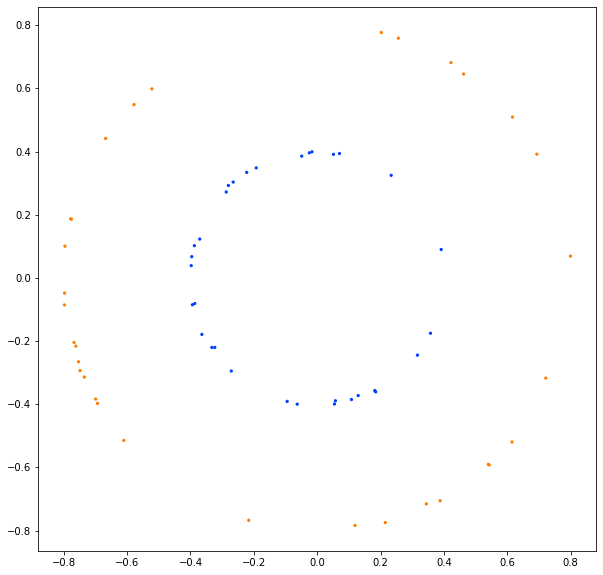
\includegraphics[width=0.475\textwidth]{figures/labeled_2_circles.png}}
\hfill
\onslide<2->{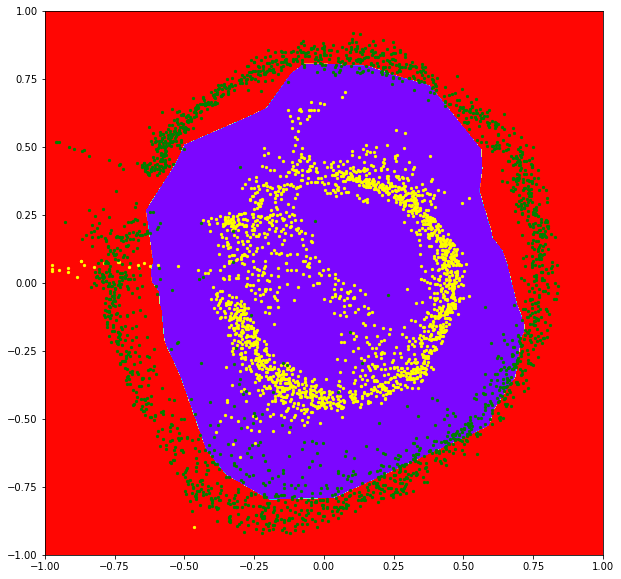
\includegraphics[width=0.475\textwidth]{figures/trained_2_circles_semisup.png}
{\scriptsize Note: 32 labeled points, 1024 unlabeled points}}

\end{frame}

\begin{frame}{VMoNF: Experiments - MNIST}
\protect\hypertarget{vmonf-experiments---mnist}{}

\centering

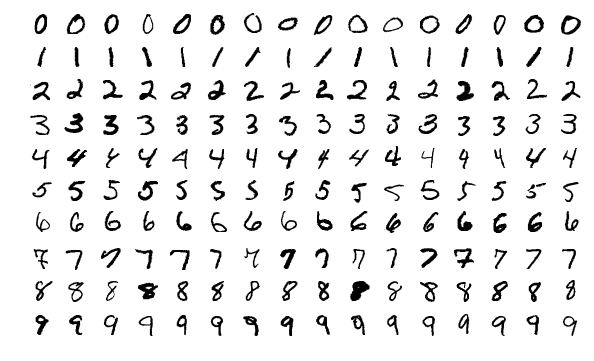
\includegraphics[width=0.7\textwidth]{figures/trained_mnist.png}

\end{frame}

\hypertarget{conclusions}{%
\section{Conclusions}\label{conclusions}}

\begin{frame}{Conclusions and Future Work}
\protect\hypertarget{conclusions-and-future-work}{}

\begin{fitemize}{0pt}{20pt}
    \onslide<1->{\item Similar work is being pursued and published in prominent venues: \mycite{RAD}, \mycite{semisuplearning_nflows}}
    \onslide<2->{\item Investigate the effect of a consistency loss regularization term}
    \onslide<3->{\item Weight-sharing between components}
    \onslide<4->{\item Balance between complexities}
    \onslide<5->{\item (Controlled) component anihilation}
\end{fitemize}

\end{frame}

\begin{frame}{}
\protect\hypertarget{section}{}

\centering

Thank you!

\end{frame}

\end{document}
